\documentclass[conference]{IEEEtran}
\IEEEoverridecommandlockouts
\usepackage{algorithmic}
\usepackage[ruled]{algorithm2e}
\usepackage[backend=bibtex,style=ieee,natbib=true]{biblatex}
\usepackage{graphicx}
\usepackage{pifont}  % for the checkmark/crossmark
\newcommand{\cmark}{\ding{51}}
\newcommand{\xmark}{\ding{55}}
\usepackage{textcomp}
\usepackage{xcolor}
\usepackage{xurl}

\addbibresource{main.bib}

\begin{document}

\title{
    COMPSCI 402 --- Artificial Intelligence\\
    Final Report\\
    The Development and Outlook of AI Techniques in The Field of
    Practical Federated Learning on Mobile Devices
}

\author{
    \IEEEauthorblockN{Sichang He}\\
    sichang.he@dukekunshan.edu.cn
}

\maketitle

\begin{abstract}
% TODO: Insert a very brief paragraph to summarize your essay
\end{abstract}

\section{Introduction}

% Briefly introduce your understanding of AI,

Artificial intelligence (AI) refers to
artificial machineries that resembles human intelligence,
either in terms of their functionality or behavior.
These machineries, or intelligent agents,
are not limited to,
but are commonly implemented in the form of computer software programs
running on general-purpose computer hardware.

Machine learning (ML), a significant subfield in AI,
focuses on the study of intelligent agents that can
adapt to previously unseen situations based on historical data.
During this adaptation process,
an intelligent agent analyzes data from the past to
prepare its abilities,
also known as ``learning'', or ``training''.
The data used is respectively referred to as ``training data''.
Upon completion of training,
the agent would be able to make predictions or inferences,
even when facing previously unobserved situations.
To implement ML, the common approach is to build models,
programs that implement mathematical functions.
These models are then trained by adjusting their function parameters.

% provide an overview of the application of the AI in your research area.
% For example, you can discuss the current development trend and
% provide a roadmap of the development of AI techniques in your research area.

Federated learning (FL), first proposed in 2016, is an ML technique that
allows distributed intelligent agents to collaborately train a model using
their local data~\cite{mcmahan2017communication,yang2019federated}.
These private data are kept local,
therefore FL is suitable for scenarios where
the training data cannot be shared to a central agent due to
privacy restrictions.

The growing demand for ML model training in various business sectors,
the rising awareness of data privacy concerns among individuals,
and the improvements in government laws have spurred
the popularity of FL applications.
It is a compelling option that enables companies to train ML models using
user data without violating some of the privacy regulations.

FL finds relevance in situations where
individual intelligent agents' private data are at the core of an ML problem,
a common scenario in FL applications on mobile devices.
Early practical applications of FL,
as proposed in~\cite{bonawitz2019towards},
included item selection and ranking,
personalized content recommendations,
and next-word prediction for smart keyboard on mobile devices.
In all these applications,
the private data from the users' interactions with
the keyboard are essential for the problems.
Since then, a significant portion of practical applications of FL have been
revolved around mobile devices,
including vision-based product quality inspection~\cite{bharti2022edge} using
an iOS application and
SMS spam classification on Android devices~\cite{sriraman2022device}.
The wide reach to private data from personal mobile devices makes
them the ideal participants for many FL applications.

Despite the theoretical advantages of FL on mobile devices,
the practical deployment of its applications are still limited.
The concept of FL was introduces as early as 2016~\cite{mcmahan2017communication},
and the its first effective and widely recognized application
was announced in 2019~\cite{bonawitz2019towards},
yet, even in 2023, practical FL applications on mobile devices remain scarce.
This scarcity can be attributed to multiple challenges practical FL encounters,
including privacy and security concerns,
training efficiency and performance issues,
and heterogeneity problems~\cite{wen2023survey}.

To approach practical FL on mobile devices,
we first present a general overview of the FL procedure in
Section~\ref{sec:general-procedure}.
Then, we analyze and address three key challenges encountered in
FL on mobile devices—scheduling (Section~\ref{sec:scheduling}),
communication (Section~\ref{sec:communication}), and
on-device training (Section~\ref{sec:on-device}).
Finally, we discuss additional challenges and
provide a potential roadmap for practical FL on mobile devices in
Section~\ref{sec:discussion}.

\section{The General Procedure of Federated Learning on Mobile Devices}

\label{sec:general-procedure}

\begin{algorithm}
  \caption{The General Procedure of Federated Learning}
  \label{algo:general-procedure}
  \ForEach{Training iteration}{
    Distribute the global model to all clients\;
    \ForEach{Client}{
      Train the local model using local training data\;
      Send the trained local model back to the central server\;
    }
    The central server aggregates all local models into a new global model\;
  }
\end{algorithm}

Generally, FL involves a distributed system that
consists of two parties of intelligent agents—the
clients and the central server.
The process typically unfolds through a series of training iterations,
with four phases per iteration,
as illustrated in Algorithm~\ref{algo:general-procedure}.
From the perspective of the ML models being trained,
in each iteration,
the central server orchestrates the distribution of the global model
to the clients.
Subsequently, the clients train the global model locally using
their individual local training data.
Following local training,
clients transmit their trained local models back to the central server.
Finally, these local models are aggregated to generate an updated global model,
and the process is repeated for successive iterations.
In the context of FL on mobile devices,
clients are typically mobile applications running on Android or iOS devices,
and the central server is a remote server on the Internet,
as depicted in Fig.~\ref{fig:general-fl}.

\begin{figure}
\centerline{
    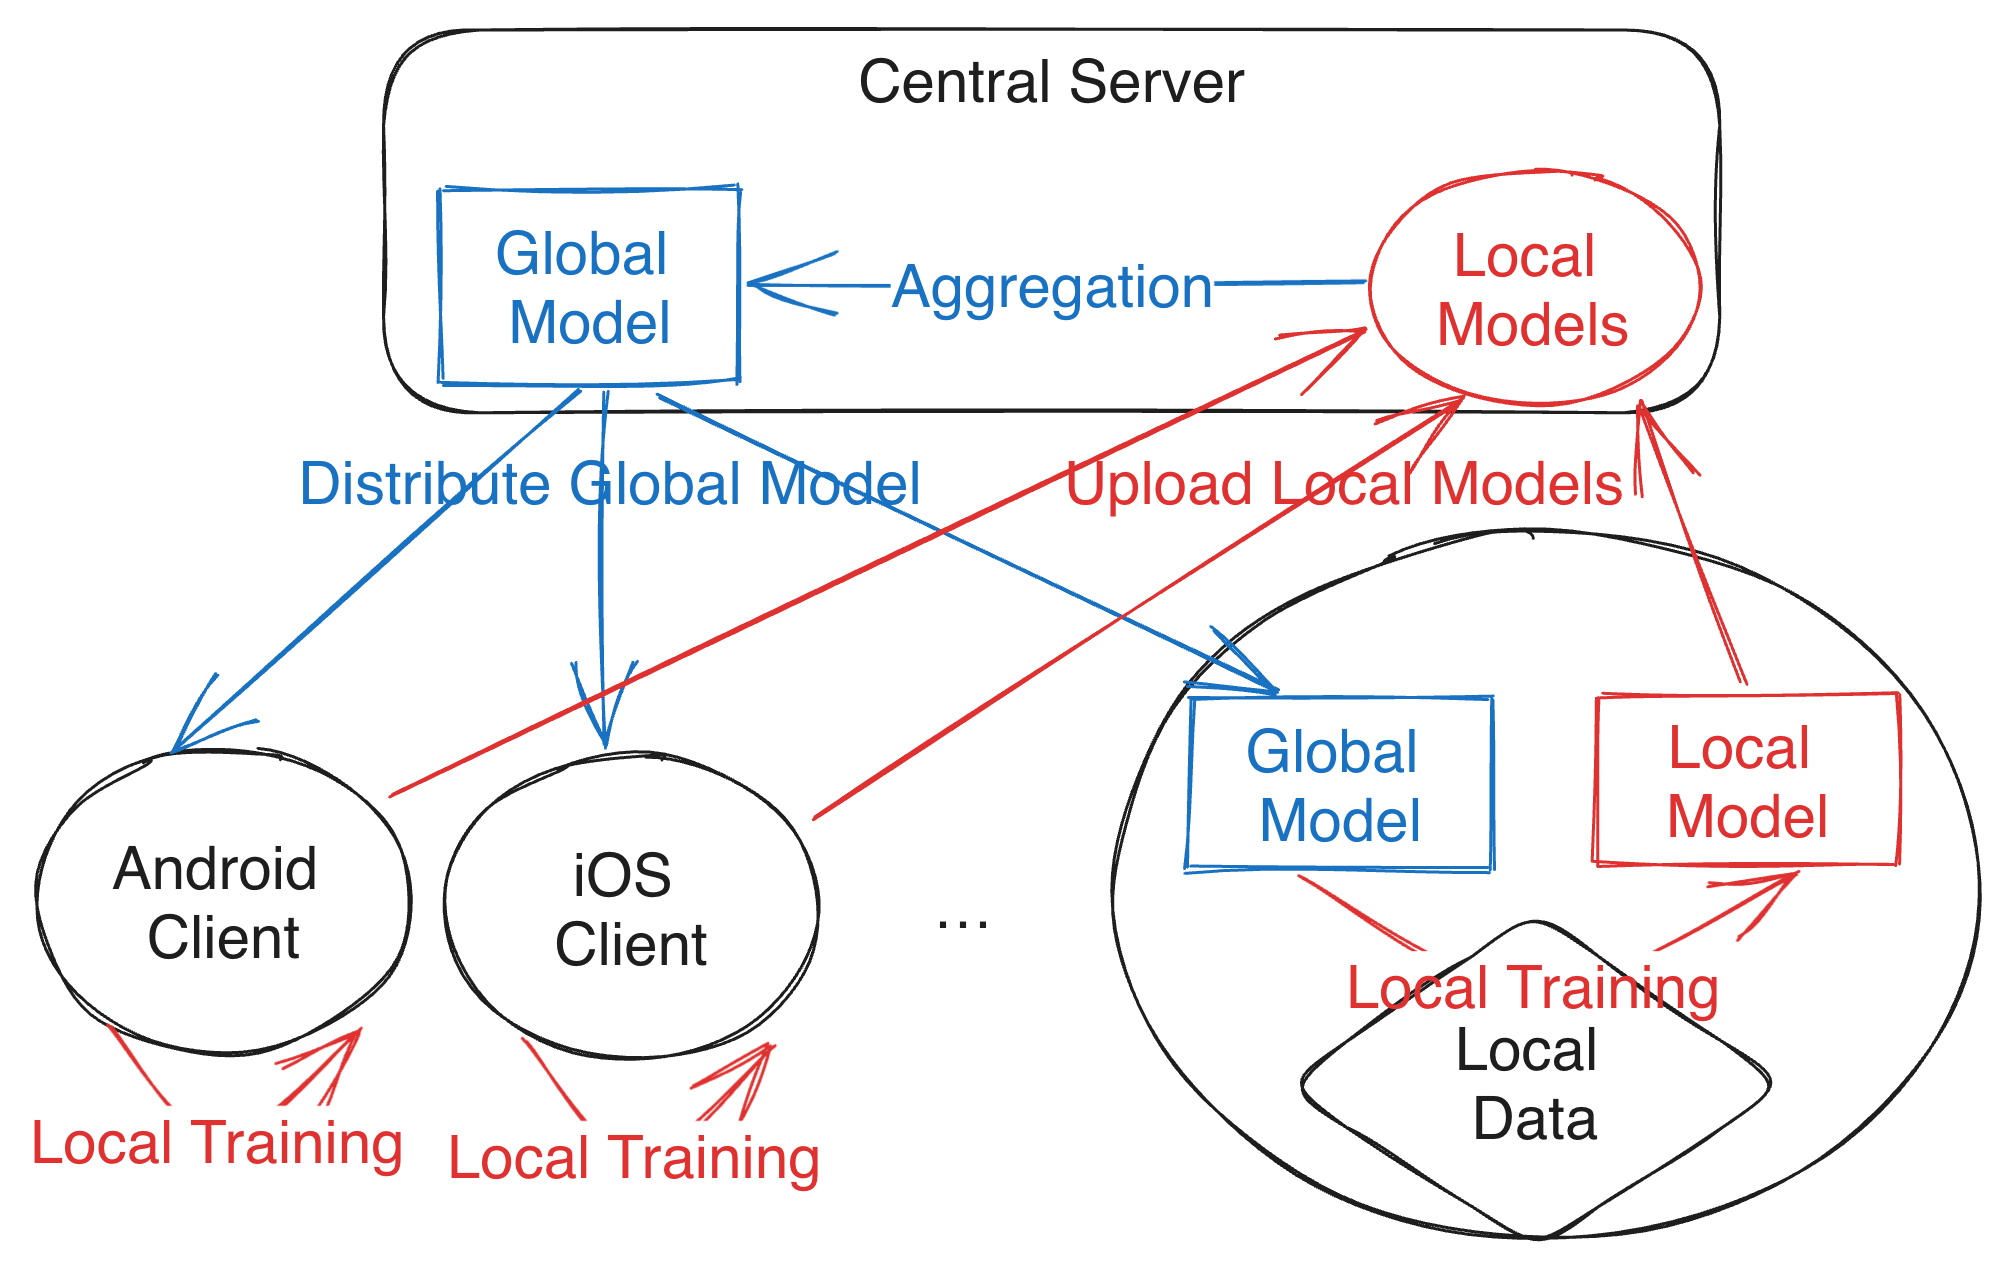
\includegraphics[width=0.5\textwidth]{general-fl.png}
}
\caption{General Procedure of FL for Mobile Devices.}
\label{fig:general-fl}
\end{figure}

The specific implementations of FL on mobile devices exhibit variations,
but they all share a common foundation,
which we delve into in the following.

\subsection{The FedAvg Algorithm}

\newcommand{\FedAvg}{\texttt{FedAvg}}

The pioneering FL algorithm, \FedAvg{},
was presented with FL itself~\cite{mcmahan2017communication}.
It also stands as the most typical FL algorithm,
with many of its aspects regarded as the standard FL procedures.
Numerous other FL scheduling strategies are slightly modified version of
\FedAvg{} and preserves its core principles.

In \FedAvg{},
we assume a fixed number of $K$ clients,
each client with $k$ a fixed partition $P_k$ of
the overall training data ($k \in \{1, 2, \dots, K\}$) as their local data.
For efficiency,
in each iteration $t$ of the training process,
the central server randomly samples $C$ clients for local training.
Each selected client $k$ receives the parameters $w^{(t)}$ of
the latest global model from the server,
and then train the model locally using their local data $P_k$
to produce a new local model.
The objective of this local training process is to minimize the loss $L$ of
the model with parameters $w_k$ for partition $P_k$:
\begin{equation}
    \min_{w_k} L(P_k;w_k).
\end{equation}
The local training is scheduled for a fixed number of $E$ epochs,
ultimately yielding an updated set of weights $w_k^{(t+1)}$ for
each selected client $k$.

To aggregate the local models into a global model
optimized for the entire training dataset $\bigcup_k P_k$,
the objective for the global model entails
a weighted average of local losses:
\begin{equation}
    \min_{w} \frac{\sum_k |P_k|L(P_k;w)}{\sum_k |P_k|}
\end{equation}
where $|P_k|$ is the size of partition $P_k$.
To approach this objective,
\FedAvg{} aggregates the parameters of local models by
computing their weighted average:
\begin{equation}
    w^{(t+1)}=\sum_k \frac{|P_k|}{\sum_k |P_k|}w_k^{(t+1)}.
\end{equation}

The above iteration step is repeated multiple times until
model convergence or experiment termination.

\FedAvg{} has been demonstrated to be effective and practical
in a variety of experimental scenarios~\cite{mcmahan2017communication}.
Specifically, it was benchmarked against \verb|FedSGD|\cite{chen2016revisiting},
an earlier algorithm developed for distributed ML,
in data center settings~\cite{bonawitz2019towards}.

\subsection{The Specific Challenges of Practical Federated Learning on
Mobile Devices in the Context of FedAvg}

FL on mobile devices introduces distinct challenges compared to
FL in data center settings.
Mobile devices are a diverse set of intelligent agent hosts compared to
servers in data centers.
They exhibit a high degree of heterogeneity,
encompassing various hardware and software configurations.
Thus, applying \FedAvg{} to FL on mobile devices in practical scenarios
presents unique difficulties.

\subsubsection{Scheduling}

FL on mobile devices require tailored scheduling strategies.
\FedAvg{} waits for each client to complete its training task in
each iteration.
However, mobile clients differ greatly in their computational capabilities,
leading to variations in training time.
A small number of clients may lag significantly behind others,
ultimately becoming the bottleneck for the overall training process—a
phenomenon known as
``the straggler problem''~\cite{chen2020asynchronous,zheng2017asynchronous}.

The straggler problem significantly decrease the training efficiency in FL.
While strategies like backup workers have been employed to
mitigate this problem in traditional settings~\cite{chen2016revisiting},
such method is not suitable in the context of FL on mobile devices because
each client typically holds a distinct set of data.
Novel scheduling strategies are developed to
enhance the efficiency of FL on mobile devices.

\subsubsection{Communication}

FL on mobile devices faces significant challenges in effective communication.
In \FedAvg{}, all model parameters are transmitted between
clients and the central server.
In FL on mobile devices,
clients primarily connect to the server via wireless networks,
which constrains both transmission bandwidth and reliability.
Various techniques are adopted to reduce data transmission volumes
and enhance the reliability of the transmissions.

\subsubsection{On-Device Training}

The final obstacle that prevents practical FL on mobile devices is
on-device training.
To start with, training ML models on mobile devices has been
a cutting-edge technology and
is generally not well-supported across mobile platforms.
Additionally,
while \FedAvg{} assumes uniformity in model parameter formats known to
all participating agents,
mobile on-device training typically employs platform-specific ML frameworks
that diverge from those on the server.
This parameter misalignment challenge is compounded when
mobile clients operate on distinct platforms with
different ML frameworks.
Addressing the on-device training issue entails
experimentation with various ML frameworks,
and in some cases,
the development of custom training implementations tailored for
specific FL frameworks

\section{Customizations in Federated Learning Scheduling Strategies for
    Mobile Devices
}

\label{sec:scheduling}

The inherent heterogeneity of mobile devices necessitates
the adoption of tailored scheduling strategies for FL.
With the conventional FL setup like \FedAvg{} applied,
the stragglers would dictate the training efficiency of the whole system.
Moreover, the data heterogeneity among the clients also poses a challenge in
model convergence~\cite{zhang2022fedada}.
Therefore, customizations must be applied on scheduling strategies.
These customizations need to be first developed,
then tested and implemented in practice under FL frameworks.

\subsection{Developing Scheduling Strategies}

The typical settings for the original \FedAvg{} can be modified in
various ways to cater to diverse FL requirements.
For example,
client selection can be changed to a function based on
each client's properties instead of being random,
and the number of clients sampled per iteration can be made variable.
Similarly, alternative aggregation methods for local parameters
may be employed.

Various strategies have been proposed to address the straggler problem.
One approach involves implementing a timeout mechanism to exclude
straggler devices~\cite{bonawitz2019towards}.
However, this approach is not suitable for FL on mobile devices because
the inherent low performance of some devices would render
their training data permanently excluded and wasted.

\newcommand{\FedProx}{\texttt{FedProx}}
\newcommand{\TFF}{TensorFlow Federated~\cite{tff}}

Many strategies to mitigate the heterogeneity problem rely on
synchronous aggregation.
For instance,
\FedProx{}~\cite{li2020federated}
allows clients to train for different numbers of local epochs according to
their computational capabilities.
In heterogeneous settings,
\FedProx{} has demonstrated superior efficiency compared to \FedAvg{} .
It has been widely supported in FL frameworks designed for simulations and
benchmarks, such as
\TFF{},
Syft~\cite{ryffel2018generic,Ziller2021,hall2021syft}, and
LEAF~\cite{caldas2018leaf}.
Other similar optimizations such as
\verb|ef-signSGD|~\cite{karimireddy2019error},
\verb|FedAdam|~\cite{reddi2020adaptive},
and~\cite{luo2021cost} have also been explored.

\newcommand{\FedML}{FedML~\cite{he2020fedml}}
\newcommand{\Florida}{Project Florida~\cite{madrigal2023project}}

Alternatively,
as opposed to strict iterations,
the training process can adopt an
asynchronous approach~\cite{chilimbi2014project,zhu2022online,huba2022papaya}.
Asynchronous aggregation has been adopted in
FL frameworks such as \FedML{} and \Florida{}.
Semi-asynchronous FL techniques have also been explored,
such as in~\cite{sun2022fedsea}.

\subsection{Testing Scheduling Strategies}

Numerous FL frameworks have been developed for
conducting production-level FL simulations and
experimentation with scheduling strategies.
Google's \TFF{} is widely adopted as infrastructure for simulation because of
its comprehensive features.
PaddleFL\footnote{\url{
    https://github.com/PaddlePaddle/PaddleFL
}.} in PaddlePaddle~\cite{ma2019paddlepaddle} by Baidu,
FATE~\cite{liu2021fate} by Tencent, and
OpenFL~\cite{patrick2022openfl} by Intel
serve similar purpose,
offering environments for production-grade FL simulations.
Additionally,
FL benchmarks such as FedScale~\cite{lai2022fedscale} are instrumental in
comparing and identifying scheduling strategies with superior performance.

\subsection{Implementing Custom Scheduling Strategies in Practice}

\newcommand{\Flower}{Flower~\cite{beutel2020flower}}

In FL frameworks such as \FedML{} and \Flower{},
the customization of scheduling strategies on the client side is
left entirely to the users.
From a programming perspective,
these frameworks provide interfaces,
also known as abstract classes,
for custom clients to implement.
These interfaces typically encompasses methods for
local model training,
model parameter retrieval and modification,
and message handling\footnote{\url{
    https://github.com/FedML-AI/FedML/blob/9aeb0c097efc9ea7037cfe24499c3d61c81c4dca/android/fedmlsdk/src/main/java/ai/fedml/edge/FedEdgeApi.java
}.}\footnote{\url{
    https://github.com/adap/flower/blob/4df413f8a1696f643fdde27bf7bac8c33b623f56/src/kotlin/flwr/src/main/java/dev/flower/android/Client.kt
}.}\footnote{\url{
    https://github.com/adap/flower/blob/4df413f8a1696f643fdde27bf7bac8c33b623f56/src/swift/flwr/Sources/Flower/Client/Client.swift
}.}.
These interfaces greatly increases the flexibility for the users to
design and implement custom scheduling strategies,
but the responsibility of implementing these strategies can
sometimes be burdening,
especially considering that the mobile clients often need to
be implemented in Java or Swift.

On the server side,
while the customizations are typically more accessible with
open-source frameworks,
the emergence of FL as a service (FLaaS)
introduces complexity.
These FLaaS providers manage proprietary servers,
often accessible to the users through opaque APIs or
graphical user interfaces (GUIs).
For instance, \FedML{}
offers a set of Python APIs for server customization
and enables users to upload their server implementations via a web GUI.
\Florida{}, another production-ready FLaaS by Microsoft,
supports the uploading of Python scripts or .NET executables for
server aggregation functions.
While these FLaaS solutions also provide web GUI for convenience,
their customizability is often limited.

\section{Communication Strategies in Federated Learning on Mobile Devices}

\label{sec:communication}

Efficient and reliable communication is paramount in FL on mobile devices,
where network connectivity is often constrained.
Various techniques and protocols are employed to
optimize communication between mobile clients and the central server.

\subsection{Minimizing Data Transmission}

To alleviate the strain on mobile networks,
FL systems often employ strategies to reduce the amount of data transmitted.
One such approach involves transmitting only
the difference between the latest local model parameters and
the last global model\footnote{\url{
        https://ai.googleblog.com/2017/04/federated-learning-collaborative.html
}.}.
Furthermore,
Frameworks like Hermes~\cite{li2021hermes} take this concept further by
leveraging sub-networks to minimize the transmitted model parameter data.
However, implementing advanced communication techniques on mobile devices
are usually challenging due to the less accommodating nature of
mobile development environments compared to the theoretical research settings.

\subsection{Practical Implementations of the Communication Among Mobile Clients
    and the Server
}

In practice,
Remote Procedure Call (RPC) is the standard protocol of communication in
practical FL.
RPC offers flexibility by enabling clients and the server to
exchange instructions for execution on the other side,
facilitating customization of FL scheduling strategies.

The gRPC Remote Procedure Call\footnote{\url{
    https://grpc.io/
}.} is a popular choice for FL communication.
It is employed by \TFF{} and
OpenFL~\cite{patrick2022openfl} for decentralized simulations.
\Flower{} uses gRPC for the standard implementation of
its communication protocol, the Flower Protocol~\cite{beutel2020flower}.
\Florida{} provides users the flexibility to choose between
REST~\cite{Richards2006} or gRPC.

The combination of gRPC and protocol buffers (ProtoBuf)\footnote{\url{
    https://protobuf.dev/
}.} offers several advantages for communication in FL on mobile devices.
ProtoBuf is a compact binary data structures representation,
allowing for efficient transmission~\cite{popic2016performance},
which is particularly valuable under mobile devices'
often constrained network conditions.
Additionally,
gRPC and ProtoBuf are language-agnostic and
provide support for a wide range of programming languages,
facilitating their adoption on different platforms~\cite{araujo2020performance}.
As gRPC is based on HTTP/2,
it can usually bypass mobile devices' restricted firewalls and
pass through proxies~\cite{araujo2020performance},
and offers guaranteed delivery from TCP.
Being connection-based and bidirectional,
gRPC also allows the server to actively push instructions to the clients and
identify clients that have lost connection.
Features such as compact representation and bidirectional communication are
not gRPC-exclusive,
but are common in other RPCs adopted in practical FL,
making gRPC a representative example.

Besides gRPC, other RPC-based communication protocols are
also adopted by FL frameworks.
\FedML{} adopts an abstract communication layer that interfaces with
the concrete implementations.
These implementations either utilize the message passing interface
(MPI)\footnote{\url{
    https://www.mpi-forum.org/
}.} over HTTP,
or employ the MQTT protocol\footnote{\url{
    https://mqtt.org/mqtt-specification/
}.}.
Syft, another prominent player in FL,
opts for WebSockets to facilitate communication between
its network-based workers and the server~\cite{Ziller2021}.

\section{On-Device Training for Federated Learning on Mobile Devices}

\label{sec:on-device}

One of the critical challenges in FL on mobile devices is
the lack of comprehensive support for on-device training in
the majority of FL frameworks.
Notable examples, such as
\TFF{} and LEAF~\cite{caldas2018leaf},
are primarily geared towards simulations~\cite{kholod2020open}.
Even some frameworks targeting business are constrained in their mobile support,
such as PaddlePaddle~\cite{ma2019paddlepaddle} that
only offers support inference on Android.

In the few cases where FL frameworks do support on-device training,
there are serious limitations.
These FL frameworks often only support a specific mobile operating system,
or lacks support for hardware acceleration.
For instance, Table~\ref{tab:on-device} outlines the functionalities of
various FL frameworks concerning mobile on-device training.
As an exception,
\Flower{} leaves the on-device training implementation to
its users,
but provides example Android and iOS implementations\footnote{\url{
    https://github.com/adap/flower/tree/main/examples/android-kotlin
}.}\footnote{\url{
    https://github.com/adap/flower/tree/main/examples/ios
}}.


\begin{table}
\caption{Mobile On-Device Training Functionalities of
    Federated Learning Frameworks.
}
\begin{center}
\begin{tabular}{cccc}
    Functionality&Android&iOS&Hardware Acceleration\\
    \hline
    TensorFlow Federated&\xmark&\xmark&\xmark\\
    LEAF&\xmark&\xmark&\xmark\\
    PaddleFL&\xmark&\xmark&\xmark\\
    Flower&\cmark$^\mathrm{a}$&\cmark$^\mathrm{a}$&\cmark$^\mathrm{a}$\\
    FedML&\cmark&\xmark&\cmark\\
    Syft&\cmark&\cmark&\xmark\\
    FedScale&\cmark$^\mathrm{b}$&\xmark&\cmark\\
    \multicolumn{4}{l}{$^{\mathrm{a}}$Up to the user to implement.}\\
    \multicolumn{4}{l}{$^{\mathrm{b}}$Only in Termux.}
\end{tabular}
\label{tab:on-device}
\end{center}
\end{table}
\subsection{First-Party Mobile Machine Learning Frameworks}

To address on-device training in FL,
most FL systems utilize existing mobile ML frameworks.
Google's TensorFlow Lite~\cite{tensorflow2015-whitepaper,abadi2016tensorflow}
for Android stands out as
a popular choice due to its flexibility and
maturity for on-device training.
For example, TensorFlow Lite is used in FLaaS frameworks such as~\cite{
    kourtellis2020flaas,katevas2022flaas}
for their Android support,
and are demonstrated in the Android examples of
Flower~\cite{beutel2020flower,mathur2021ondevice}.
In contrast, Apple's Core ML~\cite{coreml} is less prevalent because of
its relative lack of user-friendliness.
It is only adopted by a few FL frameworks such as
\Flower{} for its iOS example,
and is more commonly used for specific applications
such like vision-based quality inspection on iOS~\cite{bharti2022edge}.

Unfortunately, adopting first-party ML frameworks imposes limitations when
FL spans both Android and iOS devices.
TensorFlow Lite and Core ML are exclusive to their respective platforms,
and produce model parameters in different representations.
This discrepancy makes it challenging to aggregate local models from
Android and iOS into a single global model.
For example, to use \Flower{} to conduct FL across Android and iOS devices,
we recently developed a tedious solution that involves
ProtoBuf manipulation to obtain uniform parameter
representations~\cite{he2023fedkit}.
As a result,
FL frameworks using first-party mobile ML frameworks often have
separate training support for Android and iOS.

\subsection{Third-Party Mobile Machine Learning Frameworks}

Third-party solutions for these mobile operating systems are less commonly used
for FL on-device training,
but they offer potential solutions to the platform disparity challenge.
For example, \FedML{} employs
the MNN ML framework~\cite{jiang2020mnn,lv2022walle} by Alibaba for
on-device training on Android.
MNN claims to support Android and iOS and promises lightweight binaries.
However, MNN's documentation is
severely lacking, outdated, and confusing\footnote{\url{
    https://github.com/alibaba/MNN/tree/master/project/ios
}.}.
Also, despite their claim to support iOS,
FedML has delayed providing an iOS SDK for 15 months\footnote{\url{
    https://github.com/FedML-AI/FedML/tree/9aeb0c097efc9ea7037cfe24499c3d61c81c4dca/ios
}.}.
These issues indicate a usability problem for third-party solution for
on-device training in FL.

On the other hand,
Syft~\cite{ryffel2018generic,Ziller2021,hall2021syft} developed
its custom on-device training implementations for
both Android and iOS\footnote{\url{
    https://blog.openmined.org/announcing-new-libraries-for-fl-on-web-and-mobile/
}.}.
By using a custom implementation,
Syft ensures consistent model parameter representations across platforms,
therefore it supports FL settings that span both Android and iOS devices.
However, Syft prioritizes security and privacy over performance,
therefore these implementations greatly sacrifice
performance~\cite{ryffel2018generic}.
Furthermore, they can only utilize the CPU,
making them less practical for real-world applications of
FL on mobile devices.
Unfortunately, development on
both implementations for Android and iOS,
KotlinSyft\footnote{\url{
    https://github.com/OpenMined/KotlinSyft
}.} and SwiftSyft\footnote{\url{
    https://github.com/OpenMined/SwiftSyft
}.} has been inactive for over two years,
demonstrating the lack of interest the develop and maintain
custom third-party mobile on-device training implementations of FL.

Some rising third-party on-device training solutions are worth keeping an eye on,
but the difficulty to interface hardware on different platforms is
still an major challenge.
ONNX Runtime~\cite{onnxruntime} by Microsoft aims to
unify the ML experience on all platforms by
supporting Open Neural Network Exchange (ONNX),
an open-source format to represent deep learning
models~\cite{ParedesdelRio2020}.
However, its current implementations is limited to CPU utilization,
missing out on the massive performance improvements offered by
the hardware acceleration
from GPUs and NPUs on modern mobile devices.
This limitation restricts practical usage of ONNX Runtime.

\subsection{Not-For-Mobile Solutions}

Some systems opt for solutions not specifically designed for
mobile ML,
including web-based and UNIX-environment-based options.
For example,
TensorFlow.js is capable of running inside a browser on mobile devices or
a webview inside mobile applications~\cite{smilkov2019tensorflow}.
While this approach posed testing difficulties due to
the language limitations of JavaScript~\cite{sriraman2022device},
it is also showcased as advantageous when integrated into
a React Native application for split learning on
iOS~\cite{palanisamy2021spliteasy}.
Another example is FedScale~\cite{lai2022fedscale},
which employs Termux, a UNIX console on Android,
to run TensorFlow directly.
However, FedScale's approach is limited to benchmarking purposes and
cannot be embedded into other mobile applications in practice.

\subsection{Model Personalization}

In addition to traditional FL,
model personalization has emerged as a prominent variant.
While traditional FL focuses on training a global model,
model personalization tailors local models to each user's specific data,
making it well-suited for scenarios with
high statistical heterogeneity among users~\cite{kulkarni2020survey}.
Model personalization also alleviates some of
the restrictions and difficulties faced by traditional FL,
such as the need to train entire deep neural networks on mobile devices.
Instead, it often involves updating only the last layer of neural networks in
transfer learning,
maintaining efficiency even with deep neural networks.
Therefore, model personalization can allow for larger models to be used,
extending the reach of FL on mobile devices.

% (You can use table to summarize the features of existing methods;
% or you can conduct the comparative study by
% testing some state-of-the-art methods on your selected dataset.)

\section{Discussion}

\label{sec:discussion}

% Provide an outlook on the development of AI technology in
% your research area based on your knowledge of your research area and
% your understanding of AI.
% You can discuss some open challenges and try to
% provide the corresponding potential solutions or
% discuss the potential research directions.

From its inception in 2016,
federated learning has witnessed remarkable progress in both
theoretical exploration and concrete implementation.
These advancements have paved the way towards
practical FL applications on mobile devices.
The development in FL scheduling strategies and
the standardization of communication protocols have
significantly enhanced the theoretical foundations of FL.
Additionally,
the proliferation of open-source FL frameworks,
which are not only used for simulations and benchmarks but
also for on-device experiments,
has provided researchers with tools and algorithms to explore and
experiment with FL.
Notable among these is PySyft\footnote{\url{
    https://github.com/OpenMined/PySyft/
}.}~\cite{ryffel2018generic,Ziller2021,hall2021syft},
which has democratized FL research~\cite{sriraman2022device}.

Despite these advancements, practical FL on mobile devices still grapples with
several substantial challenges.

The most formidable roadblock to practical FL on mobile devices remains
the limited support for on-device training within popular FL frameworks.
On-device training encompasses complex tasks that
often demand reliance on platform-specific,
experimental, or
proprietary mobile FL frameworks like TensorFlow Lite and Core ML.
This creates a significant dilemma for practitioners,
and most FL frameworks opt for these platform-specific ML frameworks.
Custom training implementations like Android and iOS implementations of
Syft are constrained to CPU usage,
resulting in limited practicality.
Consequently, conducting on-device FL on mobile devices with
existing FL frameworks becomes challenging for
anyone other than the platform's vendor, such as Google or Apple.

Security remains a critical concern in FL.
Attacks to FL systems to reverse engineer the training data have been
demonstrated to be practical~\cite{sun2019really}.
Mechanism to bolster anonymity and
minimize the risk of such attacks have been proposed and implemented.
Techniques like
homomorphic encryption (HE)~\cite{wang2020homo},
secure multi-party computing (SMC)~\cite{bonawitz2016practical}, and
differential privacy
(DP)~\cite{dwork2006differential,geyer2017differentially} have been
widely adopted by production-level FL frameworks and
their effectiveness in enhancing FL security has been demonstrated.

However, real-world FL applications on mobile devices confront a fundamental
issue of trust.
Once mobile applications acquire the training data,
it becomes challenging to verify whether the data are indeed used for FL or
secretly transmitted to a central server.
Companies may well employ FL to mask their direct data collection.

The prospects for FL on mobile devices appear promising,
with active theoretical research offering hope that scheduling,
communication, and security challenges can be addressed effectively.
Yet, the fundamental obstacle of control in the mobile operating system domain
remains a formidable barrier.
Practical FL on mobile devices could continue to be dominated by
major players like Google and Apple due to
their control over on-device training and local data collection.

The path forward involves fostering an increasingly open FL community to
maintain the public availability of FL frameworks.
This is vital in countering the dominance of operating system vendors who
wield significant influence over FL on mobile devices.
While the future is uncertain,
a collaborative and transparent FL community may hold the key to
overcoming these challenges and unlocking the potential of FL on mobile devices.

\printbibliography

\end{document}
